\section{Anleggets Virkemåte}
\thispagestyle{fancy}

\section{Aktiv slam - Sequencing Batch Reaktor(SBR)} 
SBR står for Sequence Batch Reactor. På anlegget er det nytta SBR-teknologi, en reinsemetode basert på aktiv slam der alle prosessar føregår i same reaktortank. 
Reaktor nyttar biologisk reinsing for å koagulere og fjerne ikkje sedimenterbare partiklar og stabilisere organisk materiale. Avløpsvatn tilførast reaktor i «batcher» for å bli reinsa og uttappa. 
Kvar avløps-batch går igjennom ein reaktorsekvens som består av fem delsekvensar:

\begin{itemize}
    \item Pause: \newline Reaktoren venter til det er behov for kapasitet.
    \item Innpumping: \newline Reaktoren mottar avløpsvatn frå mottakstanken. 
    \item Reaksjon: \newline Reaktoren luftast for å tilføre oksygen til mikroorganismane som igjen bryter ned organisk materiale, 
    og næringsstoffet som nitrogen og fosfor.
    \item Sedimentering: \newline 
    I sedimenteringsfasen skilast dei tyngre partiklane frå vatnet ved hjelp av gravitasjon. 
    Blåser og alle ventiler stengast i denne fasen for å oppnå rolege og stabile sedimenteringsforhold. Dette gir lave konsentrasjonar av suspendert stoff i avløpet.
    \item Uttapping: \newline Reinsa vatn drenerast mot resipient
\end{itemize}

\begin{figure}[htbp]
    \centering
    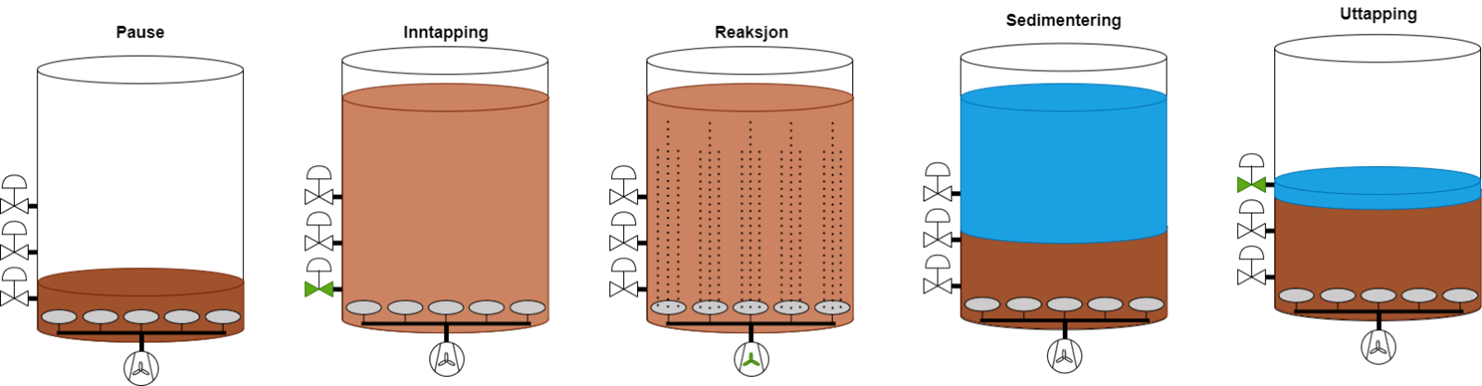
\includegraphics[width=1\textwidth]{Figurar/SBR-Prosessen.png}
    \caption{SBR-Prosessen}\label{fig:SBR-prossessen}
\end{figure}
    